\chapter{Architettura hardware}
%\markboth{Introduzione}{Introduzione}
\label{cap:architettura}

In questo capitolo viene descritta in dettaglio la componentistica hardware utilizzata per l'implementazione del gioco.

\section{Unità di elaborazione}
Sia l'elaborazione dei dati trasmessi dal robot mediante che la definizione dei comportamenti del robot in base alle logiche di gioco sono gestiti da un elaboratore esterno. Inoltre, l'elaboratore viene utilizzato dal giocatore per controllare lo stato del gioco (punteggio, tempo rimanente, ...) e per gestire l'avvio dello stesso.

\section{Il robot}

%TODO bisogna dire che per l'interpretazione dei pacchetti in arrivo è stato fatto reversing da un vecchio progetto etc etc etc?

L'attore principale del gioco è il robot autonomo \emph{Spykee}, un modello commerciale della Meccano \cite{spykeeweb}, disponibile nel laboratorio di Intelligenza Artificiale e Robotica (AIRLab) del Politecnico di Milano. Questo modello è già stato utilizzato con successo in precedenti progetti nell'ambito dei Robogame\footnote{in particolare nelle varie versioni di Robowii, l'ultima delle quali è descritta in \cite{robowii}}.

Spykee si muove tramite due cingoli (con tecnica differential drive) ed è dotato di una telecamera che permette di catturare immagini in formato \verb|JPEG| con una risoluzione di $320 \times 240$ pixel e a circa $20$ frame al secondo. Per comunicare con il computer che effettua il controllo, il robot crea all'accensione una rete \verb|Wi-Fi| ad-hoc.

\paragraph{Aggiunte hardware} A partire da quanto già realizzato in precedenti progetti, il robot è stato dotato di ulteriori sensori che lo rendono adatto all'utilizzo all'interno del gioco. Tutti i componenti hardware aggiunti al robot comunicano con l'unità di elaborazione tramite un collegamento wireless di tipo Zigbee (utilizzando un modulo XBee della Digi). Il protocollo Zigbee, è caratterizzato da una bassa velocità di trasmissione (comunque ampiamente sufficiente per gli scopi del progetto), ma da una buona facilità di utilizzo, specialmente in ambito embedded: viene infatti utilizzato come un collegamento seriale punto-punto tra i due dispositivi connessi.

Per interfacciare i vari dispositivi con il canale Zigbee è stata montata sul robot una scheda STM32F4 Discovery Board della ST, dotata di un microcontrollore ARM Cortex M4. Il firmware che permette di controllare l'hardware aggiunto al robot è stato sviluppato per il sistema operativo ChibiOS/RT\cite{chibios}.
L'utilizzo di un sistema operativo per microcontrollori permette di utilizzare astrazioni quali thread e mutex, nonché di astrarre l'hardware sottostante, consentendo quindi una certa modularità (isolando ogni funzione in un thread indipendente) e quindi un rapido sviluppo del firmware.

\begin{figure}[h]
\centering
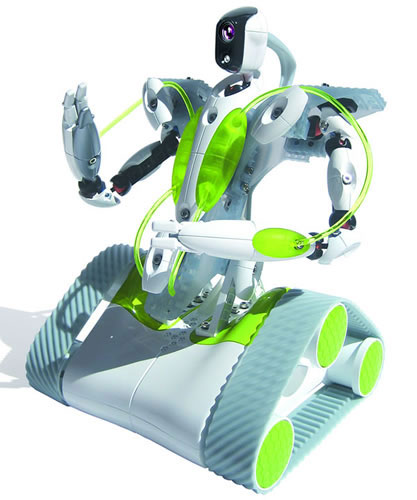
\includegraphics[scale=0.4]{images/spykee}
\caption{Il robot Spykee utilizzato nel progetto}
\end{figure}

\paragraph{Sonar e led} Il robot è stato dotato di quattro sonar MaxSonar(R)-EZ della MaxBotix, uno per ognuno dei punti cardinali (nord, sud, ovest, est), che permettono di rilevare, e quindi evitare, eventuali ostacoli incontrati durante il movimento del robot. L'aggiunta di questo tipo di dispositivi è necessaria in quanto il robot non è progettato per muoversi autonomamente, ma soltanto per ricevere comandi manuali. Inoltre, Spykee è stato dotato di due strisce di LED (quattro LED gialli, quattro rossi e uno verde) che permettono di mostrare alcune informazioni relative allo stato del robot e/o del gioco nel complesso.

%TODO bisogna spiegare l'interfaccia del firmware? (comandi che riceve, pinout, ...)

%TODO sistemare!
Le varie schede elettroniche sono state raccolte in una apposita scatola, e sono alimentate dal pacco batteria di Spykee tramite un regolatore di tensione, che permette di ridurre la tensione proveniente dalla batteria (circa $9$ V) a quella di $5$ V. Un apposito interruttore, posto a valle dell'interruttore di alimentazione di Spykee, permette di spegnere o accendere le aggiunte hardware.

\section{Ostacoli attivi}
%TODO questa roba è tutta da sistemare!!!
Un problema che si è posto riguarda l'implementazione delle trappole (ostacoli che modificano il comportamento del robot). A questo scopo, inizialmente si sono valutate valutate alcune soluzioni basati su meccanismi di visione artificiale, in quanto all'interno del gioco viene già utilizzata una telecamera montata sul robot.

In particolare, sono stati presi in considerazione vari tipi di codici, tra cui i ``Datamatrix'' e i tag della libreria ``ARToolkitPlus''. Purtroppo, tutti questi meccanismi hanno dato scarsi risultati in termini di velocità oppure di qualità del riconoscimento (enorme dipendenza dalle condizioni di luce, scarsi risultati in movimento, lentezza degli algoritmi, ...). Queste caratteristiche li rendono inadatti per l'utilizzo che ne deve essere fatto all'interno del gioco, pertanto le soluzioni basate sul riconoscimento di tag sono state scartate.

Una soluzione che ha fornito prestazioni migliori, pur richiedendo l'aggiunta di ulteriore hardware al robot, è l'uso di tag RFID passivi (a 125 KHz). A seguito di alcune prove, si è riscontrato che questa tecnologia è dotata delle caratteristiche necessarie all'utilizzo all'interno del gioco. Per la lettura dei tag, è stato montato sul robot un lettore (l'ID-12 della ID-Innovations), che trasmette i dati mediante un collegamento seriale a 9600 bps all'evaluation board presente sul robot. Una limitazione di questo specifico modello di lettore è la presenza di un antenna interna, che limita pesantemente il posizionamento del lettore nel robot.

\section{Torri e fabbriche}
Le torri e le fabbriche sono state realizzate semplicemente mediante dei cilindri di cartoncino di colori differenti, di dimensione tele da poter essere rilevati ed abbattuti dal robot. In particolare, si è utilizzato un cilindro di colore rosso per la torre, e tre cilindri più piccoli di colore giallo per le fabbriche. 

La base dei cilindri contiene un interruttore, normalmente chiuso quando il cilindro è appoggiato a terra. L'interruttore viene aperto all'abbattimento della torre, e permette di inviare un segnale radio (utilizzando dei comuni trasmettitori del tipo di quelli utilizzati per l'apertura dei cancelli elettrici) a un ricevitore montato sul robot, e quindi di segnalare l'abbattimento di una torre o di una fabbrica all'unità di elaborazione.

Il ricevitore montato sul robot è il RX-4M-HCS dell'Aurel, ed è dotato di quattro canali separati con uscita open-drain (corrispondenti ai quattro pulsanti presenti sui corrispondenti trasmettitori, sempre della stessa marca). Pertanto, si sono impostati i relativi ingressi del microcontrollore come ingressi pull-up. Le uscite del ricevitore possono essere impostate, durante l'associazione con i trasmettitori, sia in modalità monostabile (ossia sono attive quando l'interruttore è chiuso) che in modalità bistabile (cambiano stato alla pressione dell'interruttore). Per la nostra applicazione si è scelto di utilizzare la modalità monostabile. 